% Copyright 2004 by Till Tantau <tantau@users.sourceforge.net>.
%
% In principle, this file can be redistributed and/or modified under
% the terms of the GNU Public License, version 2.
%
% However, this file is supposed to be a template to be modified
% for your own needs. For this reason, if you use this file as a
% template and not specifically distribute it as part of a another
% package/program, I grant the extra permission to freely copy and
% modify this file as you see fit and even to delete this copyright
% notice.

\documentclass{beamer}

\usepackage{tikz, tikz-uml}
\usetikzlibrary{automata, matrix,shapes.multipart,shapes.geometric,fit,scopes,positioning}

\definecolor{blue-base}{RGB}{42, 79, 110}
\definecolor{purple-custom}{RGB}{54, 51, 119}
\definecolor{orange-custom}{RGB}{227, 164, 79}
\definecolor{yellow-custom}{RGB}{170, 142, 57}
\definecolor{green-user}{RGB}{176, 203, 31}
\definecolor{blue-user}{HTML}{008dd2}
\definecolor{red-user}{HTML}{e31e24}
% There are many different themes available for Beamer. A comprehensive
% list with examples is given here:
% http://deic.uab.es/~iblanes/beamer_gallery/index_by_theme.html
% You can uncomment the themes below if you would like to use a different
% one:
%\usetheme{AnnArbor}
%\usetheme{Antibes}
%\usetheme{Bergen}
%\usetheme{Berkeley}
%\usetheme{Berlin}
%\usetheme{Boadilla}
%\usetheme{boxes}
%\usetheme{CambridgeUS}
%\usetheme{Copenhagen}
%\usetheme{Darmstadt}
%\usetheme{default}
%\usetheme{Frankfurt}
%\usetheme{Goettingen}
%\usetheme{Hannover}
%\usetheme{Ilmenau}
%\usetheme{JuanLesPins}
%\usetheme{Luebeck}
\usetheme{Madrid}
%\usetheme{Malmoe}
%\usetheme{Marburg}
%\usetheme{Montpellier}
%\usetheme{PaloAlto}
%\usetheme{Pittsburgh}
%\usetheme{Rochester}
%\usetheme{Singapore}
%\usetheme{Szeged}
%\usetheme{Warsaw}

\title{ADT PLM}

% A subtitle is optional and this may be deleted
\subtitle{Programmer's Learning Machine}

\author{Matthieu~Nicolas}

\date{COAST meeting, 2016-02-12}

\subject{Theoretical Computer Science}

\AtBeginSection[]
{
  \begin{frame}<beamer>{Outline}
    \tableofcontents[currentsection]
  \end{frame}
}

\begin{document}

\begin{frame}
  \titlepage
\end{frame}

\begin{frame}{Outline}
  \tableofcontents
  % You might wish to add the option [pausesections]
\end{frame}

\section{Presentation of PLM}

\subsection{Purposes}

\begin{frame}{Presentation of PLM}{Purposes}
  \begin{itemize}
  \item {
    Application to learn programming.
    \pause
  }
  \item {
    Allows students to progress at their own speed...
    \pause
  }
  \item {
    ... while the teacher helps the ones having trouble.
    \pause
  }
  \item {
    Used at TELECOM Nancy since 2008.
  }
  \end{itemize}
\end{frame}

\subsection{Demo}

\begin{frame}{Presentation of PLM}{Quick demo}
  \begin{center}
    \href{https://plm.telecomnancy.univ-lorraine.fr}{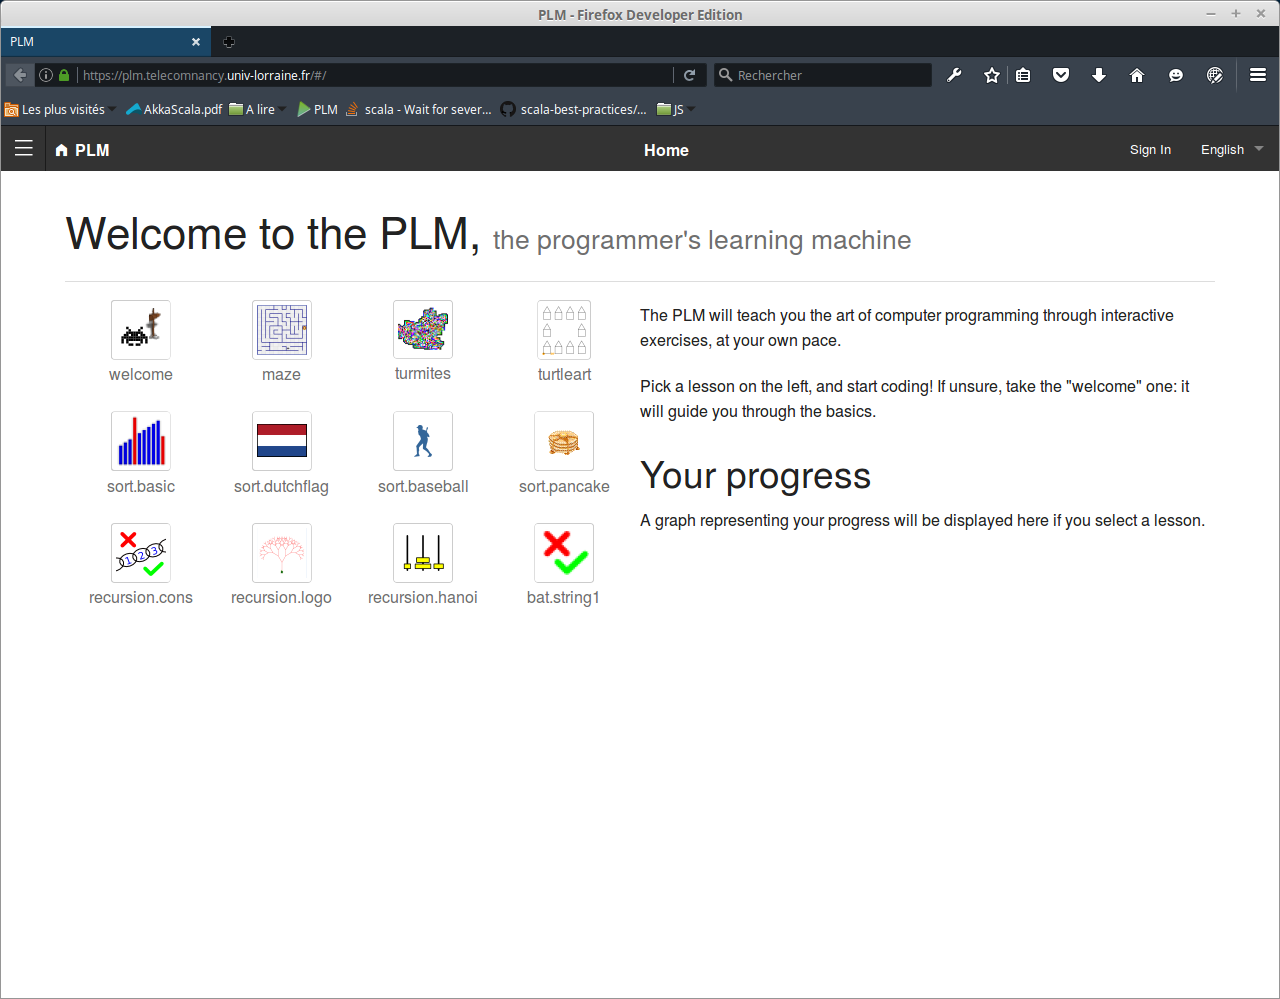
\includegraphics[scale=0.16]{img/screen-webPLM-1.png}}
    \begin{itemize}
    \item Available at \url{https://plm.telecomnancy.univ-lorraine.fr}
    \end{itemize}
  \end{center}
\end{frame}

\subsection{About PLM}

% QUESTION: Need slides for these infos or talk about them in the video?
\begin{frame}{Presentation of PLM}{12 lessons, 200 exercises}
  \begin{center}
    \includegraphics[scale=0.18]<1>{img/maze.png}
    \includegraphics[scale=0.18]<2>{img/hanoi.png}
    \includegraphics[scale=0.18]<3>{img/logo.png}
  \end{center}
\end{frame}

\begin{frame}{Presentation of PLM}{Languages and programming languages}
  \begin{itemize}
    \item {
      Available languages:
      \begin{itemize}
      \item English
      \item French
      \item Brazilian Portuguese
      \end{itemize}
    }
    \item[~]
    \item {
      Supported programming languages:
    }
  \end{itemize}
  \begin{center}
    
\includegraphics[scale=0.16]{img/java.png}
    ~
    
\includegraphics[scale=0.4]{img/scala.png}
    
\includegraphics[scale=0.18]{img/python.png}
  \end{center}
\end{frame}

\subsection{Architecture}

\begin{frame}{Presentation of PLM}{Application's architecture}
  \begin{center}
    \begin{tikzpicture}[
      scale=1,
      block/.style={
        rectangle, rounded corners=9pt,
        text width=8em,
        text centered,
        minimum height=3em,
        draw=black!50,
        fill=black!20
      },
      oauth/.style={
        block,
        color=white,
        fill=purple-custom
      }
    ]

      \node (user) { 
\includegraphics[scale=0.05]{img/user.pdf} };

      \node[block, right=1.5 of user, align=center] (webPLM) {webPLM\\(centralized/local)};

      \node[block, right=1.5 of webPLM] (plm-data) { PLM-data };

      % OAuth-providers
      \node[oauth, scale=0.5, below=1.5 of user] (plm-accounts) { PLM-accounts };
      \node[scale=0.5, below=0.3 of plm-accounts] (google) { 
\includegraphics[scale=0.1]{img/google-logo.png} };
      \node[scale=0.5, below=0.3 of google] (github) { 
\includegraphics[scale=0.1]{img/github-logo.png} };
      \node[draw=purple-custom, densely dotted, fit=(plm-accounts) (google) (github)] (oauth-providers) {};
      \node[color=purple-custom, below=0.1 of oauth-providers] {OAuth-providers};

      \node[block, below=2.5 of plm-data] (plm-profiles) { PLM-profiles };

      \path[<->, shorten >=3pt, shorten <=3pt]
        (user) edge (webPLM)
        (user) edge node[left, scale=0.6] {authentificate} (oauth-providers)
        (webPLM) edge (plm-data)
        (webPLM) edge[bend right] node[above right, align=center, xshift=-5, scale=0.6] {retrieve user's \\ preferences} (plm-profiles.west)
        (webPLM) edge[bend left] node[below right, align=center, yshift=-15, xshift=-25, scale=0.6]  {validate \\ authentification} (oauth-providers.east);

    \end{tikzpicture}
  \end{center}
\end{frame}

\begin{frame}{Presentation of PLM}{A word about PLM-data}
  \begin{itemize}
  \item { 
    Keep track of the users' progress...
    \pause
  }
  \item ... using a git repository
  \item[~]
  \end{itemize}
  \begin{center}
    
\includegraphics[scale=0.1]{img/git.png}
  \end{center}
\end{frame}

\begin{frame}{Presentation of PLM}{How does it work?}
  \begin{itemize}
  \item { 
    Store users' code versions
    \pause
  }
  \item {
    Store users' actions as commit messages
    \begin{center}
      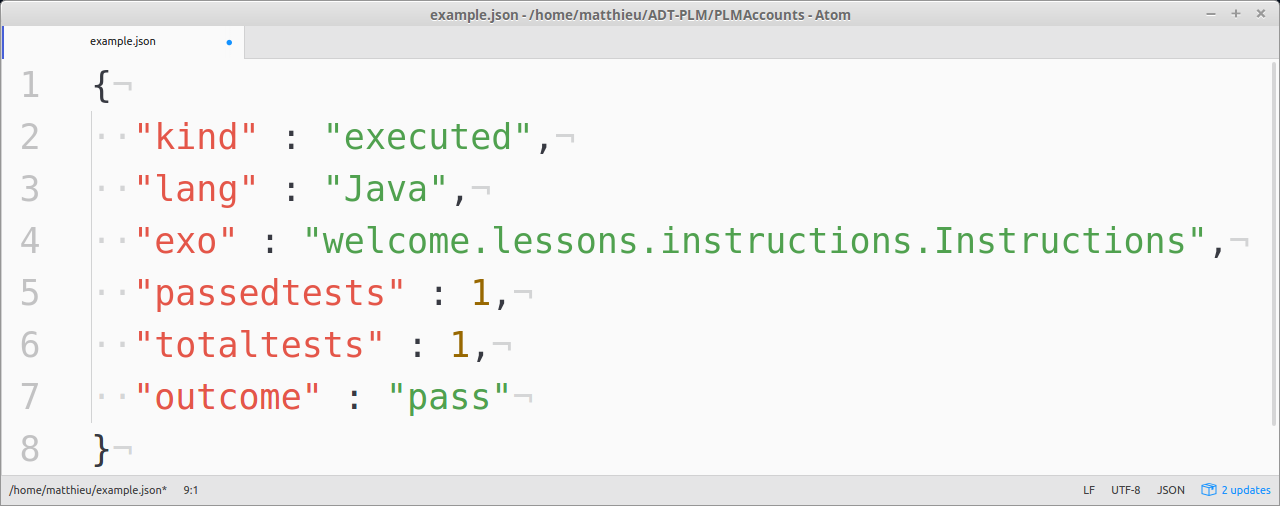
\includegraphics[scale=0.2]{img/commit.png}
    \end{center}
    \pause
  }
  \item {
    Working in anonymous branches
  }
  \item {
    Branches pushed to a \textbf{GitHub} repo
  }
  \end{itemize}
\end{frame}

\subsection{Targets}

\begin{frame}{Presentation of PLM}{Targets}
  \begin{itemize}
  \item {
    Students obviously
    \begin{itemize}
    \item {
      More teaching content
    }
    \item {
      Gamification
    }
    \end{itemize}
    \pause
  }
  \item {
    But also teachers
    \begin{itemize}
    \item {
      Keep track of the students' progress
    }
    \item {
      Adapt content to their needs
    }
    \item {
      Able to add their own exercises
    }
    \pause
    \end{itemize}
  }
  \item {
    And researchers
    \begin{itemize}
    \item {
      To an experimental teaching platform
    }
    \item {
      How to detect students having difficulties?
    }
    \item {
      What are the most common errors?
    }
    \end{itemize}
  }
  \end{itemize}
\end{frame}

\section{To a web app}

\subsection{Goals}

\begin{frame}{To a web app}{Evolution of the project}
  \begin{itemize}
    \item {
      Formerly a fat client
      \begin{itemize}
        \item { Written in Java }
      \end{itemize}
      \pause
    }
    \item[~]
    \item {
      Switch to a web application
      \begin{itemize}
        \item { Server implemented in Scala using \emph{PlayFramework} }
        \item { User interface written in Javascript using \emph{AngularJS} and \emph{Foundation} }
      \end{itemize}
    }
  \end{itemize}
  \begin{center}
    
\includegraphics[scale=0.05]{img/play-logo.png}
    ~
    
\includegraphics[scale=0.1]{img/foundation-angular.png}
  \end{center}
\end{frame}

\begin{frame}{To a web app}{Motivations}
  \begin{itemize}
  \item {
    Want to switch to SaaS\footnote{Software as a Service}
    \begin{itemize}
    \item Easy to use
    \item Easy to update
    \item Easy to track usage data
    \end{itemize}
  }
  \item {
    More user-friendly
  }
  \item {
    Aim to setup SPOC\footnote{Small Private Online Course} and MOOC\footnote{Massive Open Online Course}
  }
  \item[~]
  \item {
    But don't have the time and means for a reboot
  }
  \end{itemize}
\end{frame}

\subsection{Server-side}

\begin{frame}{To a web app}{Refactoring PLM}
  \begin{itemize}
  \item {
    Implemented a headless version of PLM: \emph{PLM-engine}
    \begin{itemize}
    \item Provide all PLM's content and methods
    \item But without a user interface
    \end{itemize}
  }
  \end{itemize}
  \begin{center}
    \begin{tikzpicture}

      \umlemptyclass{Game}
      \umlemptyclass[x=4, y=-2]{Lesson}
      \umlemptyclass[x=8, y=-4]{Exercise}

      \begin{umlclass}[x=8, y=0]{ExerciseRunner}{}{
        + runExercise() : void}
      \end{umlclass}

      \umlunicompo[arg2=lessons]{Game}{Lesson}
      \umlunicompo[arg2=exercises]{Lesson}{Exercise}
      \umlunicompo[arg2=runner]{Game}{ExerciseRunner}
      \umluniassoc[geometry=|-, anchor1=-60, arg2=currentLesson]{Game}{Lesson}
      \umluniassoc[geometry=|-, anchor1=-120, arg2=currentExercise]{Game}{Exercise}

    \end{tikzpicture}
  \end{center}
\end{frame}

\begin{frame}{To a web app}{Implementing the server}
  \begin{itemize}
  \item {
    Designed an API over PLM-engine
  }
  \item {
    Only need to implement a controller
    \begin{itemize}
    \item Verify calls received from the client
    \item Query or command PLM-engine according to the call
    \item Send back result or acknowledgement to the client
    \end{itemize}
  }
  \end{itemize}
\end{frame}

\begin{frame}{To a web app}{Interactions between components}
  \begin{center}
    \begin{tikzpicture}[
      scale=1,
      block/.style={
        rectangle, rounded corners=9pt,
        text width=8em,
        text centered,
        minimum height=3em,
        draw=black!50,
        fill=black!20
      }
    ]

      \node (user) { 
\includegraphics[scale=0.05]{img/user.pdf} };

      \node[block, right=2 of user] (plm-actor) { PLM-actor };
      \node[block, right=2 of plm-actor] (plm-engine) { PLM-engine };

      \node[draw, densely dotted, fit=(plm-actor) (plm-engine)] (webPLM) {};
      \node[below=0.1 of webPLM] {webPLM-server};

      \path[->, shorten >=2pt, shorten <=2pt]
        (user) edge node[sloped, anchor=center, above] {\tiny API call} (plm-actor)
        (plm-actor) edge node[sloped, anchor=center, above] {\tiny query / command} (plm-engine)
        ([yshift=-0.2 cm]plm-engine.west) edge node[sloped, anchor=center, below] {\tiny send result} ([yshift=-0.2 cm]plm-actor.east)
        ([yshift=-0.2 cm]plm-actor.west) edge node[sloped, anchor=center, below] {\tiny relay result} ([yshift=-0.2 cm]user.east);
    \end{tikzpicture}
  \end{center}
\end{frame}

\begin{frame}{To a web app}{Dealing with multi-user}
  \begin{itemize}
  \item {
    \textbf{Game} is a \emph{singleton}
    \pause
  }
  \item {
    Do you remember that we store the user's session in \textbf{Game}?
  }
  \item[~] {
    \begin{center}
      \begin{tikzpicture}

        \umlemptyclass{Game}
        \umlemptyclass[x=4, y=-2]{Lesson}
        \umlemptyclass[x=8, y=-4]{Exercise}

        \begin{umlclass}[x=8, y=0]{ExerciseRunner}{}{
          + runExercise() : void}
        \end{umlclass}

        \umlunicompo[arg2=lessons]{Game}{Lesson}
        \umlunicompo[arg2=exercises]{Lesson}{Exercise}
        \umlunicompo[arg2=runner]{Game}{ExerciseRunner}
        \umluniassoc[geometry=|-, anchor1=-60, arg2=currentLesson]{Game}{Lesson}
        \umluniassoc[geometry=|-, anchor1=-120, arg2=currentExercise]{Game}{Exercise}

      \end{tikzpicture}
    \end{center}
  }
  \end{itemize}
\end{frame}

\begin{frame}{To a web app}{Removing the singleton \textbf{Game}}
  \begin{itemize}
  \item {
    Need to refactor all components accessing it
    \pause
  }
  \item[~]
  \item {Let's save it for later!}
  \item {Add \textbf{Game} as constructor's parameter}
  \end{itemize}
\end{frame}

\begin{frame}{To a web app}{Multi-user scenario}
  \begin{center}
    \begin{tikzpicture}[
      scale=1,
      block/.style={
        rectangle, rounded corners=9pt,
        text width=8em,
        text centered,
        minimum height=3em,
        draw=black!50,
        fill=black!20
      },
      user1/.style={
        block,
        fill=blue-user
      },
      user2/.style={
        block,
        fill=red-user
      },
      user3/.style={
        block,
        fill=green-user
      }
    ]
      \node (ref) {};

      \foreach \x [evaluate=\x as \dist using 1.5*\x-1] in {1,...,3}
      {
        \node[below=\dist of ref] (user-\x) { \includegraphics[scale=0.05]{img/user-\x.pdf} };

        \node[user\x, right=2 of user-\x] (plm-actor-\x) { PLM-actor };
        \node[user\x, right=2 of plm-actor-\x] (plm-engine-\x) { PLM-engine };

        \path[->, shorten >=2pt, shorten <=2pt]
          (user-\x) edge node[sloped, anchor=center, above] {\tiny API call} (plm-actor-\x)
          (plm-actor-\x) edge node[sloped, anchor=center, above] {\tiny query / command} (plm-engine-\x)
          ([yshift=-0.2 cm]plm-engine-\x.west) edge node[sloped, anchor=center, below] {\tiny send result} ([yshift=-0.2 cm]plm-actor-\x.east)
          ([yshift=-0.2 cm]plm-actor-\x.west) edge node[sloped, anchor=center, below] {\tiny relay result} ([yshift=-0.2 cm]user-\x.east);
      }

      \node[draw, densely dotted, fit=(plm-actor-1) (plm-engine-1) (plm-actor-2) (plm-engine-2) (plm-actor-3) (plm-engine-3)] (webPLM) {};
      \node[below=0.1 of webPLM] {webPLM-server};
    \end{tikzpicture}
  \end{center}
\end{frame}

% TODO: Find a better subtitle
% TODO: Complete this slide
\begin{frame}{To a web app}{Results}
  \begin{itemize}
  \item {
    Build quickly a web server from the fat client...
  }
  \item {
    ... but we also need a user interface
  }
  \end{itemize}
\end{frame}

\subsection{Client-side}

\begin{frame}{To a web app}{Adding the user interface}
  \begin{center}
    \begin{tikzpicture}[
      scale=1,
      block/.style={
        rectangle, rounded corners=9pt,
        text width=8em,
        text centered,
        minimum height=3em,
        draw=black!50,
        fill=black!20
      }
    ]

      \node (user) { 
\includegraphics[scale=0.05]{img/user.pdf} };
      \node[right=0.1 of user] (browser) { 
\includegraphics[scale=0.015]{img/firefox.png} };
      \node[block, right=1.5 of browser, text width=2em] (UI) {UI};

      \node[block, right=1.5 of UI, text width=4em] (plm-actor) { PLM-actor };
      \node[block, right=2 of plm-actor, text width=4em](plm-engine) { PLM-engine };

      \node[draw, densely dotted, fit=(plm-actor) (plm-engine)] (webPLM) {};
      \node[below=0.1 of webPLM] {webPLM-server};

      \path[->, shorten >=2pt, shorten <=2pt]
        (browser) edge node[sloped, anchor=center, above] {\tiny user's action} (UI)
        (UI) edge node[sloped, anchor=center, above] {\tiny API call} (plm-actor)
        (plm-actor) edge node[sloped, anchor=center, above] {\tiny query / command} (plm-engine)
        ([yshift=-0.2 cm]plm-engine.west) edge node[sloped, anchor=center, below] {\tiny send result} ([yshift=-0.2 cm]plm-actor.east)
        ([yshift=-0.2 cm]plm-actor.west) edge node[sloped, anchor=center, below] {\tiny relay result} ([yshift=-0.2 cm]UI.east)
        ([yshift=-0.2 cm]UI.west) edge node[sloped, anchor=center, below] {\tiny update view} ([yshift=-0.2 cm]browser.east);
    \end{tikzpicture}
  \end{center}
\end{frame}

% TODO: Find a subtitle
\begin{frame}{To a web app}{}
  \begin{itemize}
    \item Have to translate user's actions into API calls
    \item Have to re-implement PLM-engine's data models
  \end{itemize}
\end{frame}

\section{Assessment of user's code}

\subsection{Challenges}

\begin{frame}{Assessment of user's code}{Limits}
  \begin{itemize}
  \item {
    Run on the same machine, same JVM
    \pause
  }
  \item[~]
  \item {
    How to protect ourselves from users' rookie mistakes?
    \begin{itemize}
    \item {
      Infinite loops
    }
    \end{itemize}
    \pause
  }
  \item {
    And from more malicious "mistakes"?
    \begin{itemize}
    \item {
      Infinite thread creation
    }
    \item {
      Endless file creation
    }
    \end{itemize}
    \pause
  }
  \item {
    And from \emph{System.exit(whatever)}?
    \pause
  }
  \item[~]
  \item {
    Scalability issues
  }
  \end{itemize}
\end{frame}

\subsection{Extraction of the execution component}

\begin{frame}{Assessment of user's code}{Chosen solution}
  \begin{itemize}
    \item Delegate execution to workers
  \end{itemize}
  \begin{center}
    \begin{tikzpicture}[
      scale=1,
      block/.style={
        rectangle, rounded corners=9pt,
        text width=8em,
        text centered,
        minimum height=3em,
        draw=black!50,
        fill=black!20
      },
      judge/.style={
        block,
        text width=4em
      }
    ]

      \node (user) { 
\includegraphics[scale=0.05]{img/user.pdf} };

      \node[block, right=2 of user] (plm-actor) { PLM-actor };
      \node[block, right=2 of plm-actor] (plm-engine) { PLM-engine };

      \node[draw, densely dotted, fit=(plm-actor) (plm-engine)] (webPLM) {};
      \node[above=0.1 of webPLM] {webPLM-server};

      \node[judge, below=2 of webPLM] (judge) {Worker 2};
      \node[right=of judge] (judge-2) {...};
      \node[judge, left=of judge] (judge-3) {Worker 1};
      \node[draw, densely dotted, fit=(judge-2) (judge) (judge-3)] (judges) {};
      \node[below=0.1 of judges] {Workers};

      \path[->, shorten >=2pt, shorten <=2pt]
        (user) edge node[sloped, anchor=center, above] {\tiny API call} (plm-actor)
        (plm-actor) edge node[sloped, anchor=center, above] {\tiny query / command} (plm-engine)
        ([yshift=-0.2 cm]plm-engine.west) edge node[sloped, anchor=center, below] {\tiny send result} ([yshift=-0.2 cm]plm-actor.east)
        ([yshift=-0.2 cm]plm-actor.west) edge node[sloped, anchor=center, below] {\tiny relay result} ([yshift=-0.2 cm]user.east)
        ([xshift=3]webPLM.south) edge node[right] {\tiny delegate execution} ([xshift=20]judges.north)
        ([xshift=14]judges.north) edge node[left] {\tiny send result} ([xshift=-3]webPLM.south);
    \end{tikzpicture}
  \end{center}
\end{frame}

\begin{frame}{Assessment of user's code}{The judges}
  \begin{itemize}
  \item Called \emph{Judges} in the litterature
  \item Use PLM-engine as well
  \item[~]
  \item {
    Workflow:
    \begin{itemize}
    \item Retrieve an execution request
    \item Parse the request to extract parameters
    \item Configure PLM-engine according to them
    \item Run the user's code
    \item Send back result to webPLM
    \end{itemize}
  }
  \end{itemize}
\end{frame}

\begin{frame}{Assessment of user's code}{Message queues}
  \begin{itemize}
    \item {
      Message-driven architecture
    }
    \item {
      Loosely coupled system
    }
    \item {
      \alert<2> {Asynchronous}/Synchronous 
    }
    \item {
      Help to implement:
      \begin{itemize}
        \item Producer/Consumer pattern
        \item \alert<2> {Request/Response pattern}
      \end{itemize}
    }
    \item {
      Different reliability patterns of the message processing:
      \begin{itemize}
        \item \alert<2> {Only one worker}
        \item At least one worker
        \item All workers
      \end{itemize}
    }
    \item {
      Easy to scale
    }
  \end{itemize}
\end{frame}

\begin{frame}{Assessment of user's code}{Architecture with judges}
  \begin{center}
    \begin{tikzpicture}[
      scale=1,
      block/.style={
        rectangle, rounded corners=9pt,
        text width=8em,
        text centered,
        minimum height=3em,
        draw=black!50,
        fill=black!20
      },
      judge/.style={
        block,
        text width=4em
      }
    ]

      \node (user) { 
\includegraphics[scale=0.05]{img/user.pdf} };

      \node[block, right=3 of user] (plm-actor) { PLM-actor };
      \node[block, right=1 of plm-actor] (plm-engine) { PLM-engine };

      \node[draw, densely dotted, fit=(plm-actor) (plm-engine)] {};
      \node[fit=(plm-actor) (plm-engine), yshift=30] {webPLM};

      \node[below=1.5 of plm-actor] (center-mq) {};

      \node[right=0.5 of center-mq] (requests-mq) { 
\includegraphics[angle=-90, scale=0.3]{img/message-queue-2.png} };
      \node[right=0.5 of center-mq, xshift=20] {\tiny \textbf{Requests}};

      \node[right=0.5 of requests-mq] (center-mq-2) {};

      \node[left=0.5 of center-mq] (reply-mq) { 
\includegraphics[angle=90, scale=0.3]{img/message-queue-2.png} };
      \node[left=0.5 of center-mq, xshift=-20] {\tiny \textbf{Reply}};
      \node[right=0.5 of center-mq-2, opacity=0.6] (reply-mq-2) { 
\includegraphics[angle=90, scale=0.3]{img/message-queue-2.png} };

      \node[judge, below=1.5 of center-mq] (judge1) {Judge 1};
      \node[judge, below=1.5 of center-mq-2] (judge2) {Judge 2};
      \node[right=0.5 of judge2] (judge3) {...};

      \node[draw, densely dotted, fit=(judge1) (judge2) (judge3)] {};
      \node[fit=(judge1) (judge2) (judge3), yshift=-35] {Judges};

      \path[->, shorten >=2pt, shorten <=2pt]
        (user) edge node[sloped, anchor=center, above] {\tiny request execution} (plm-actor)
        (plm-actor) edge node[sloped, anchor=center, above] {\tiny save result} (plm-engine)
        ([yshift=-0.2 cm]plm-actor.west) edge node[sloped, anchor=center, below] {\tiny relay results} ([yshift=-0.2 cm]user.east);
      \path[->, shorten >=2pt, shorten <=2pt]
        (plm-actor.south) edge[bend left] node[below right, xshift=5] {\tiny submit request} (requests-mq.north)
        (requests-mq.south) edge[bend left] node[right] {\tiny retrieve request} (judge1.north)
        (judge1.north) edge[bend left] node[left] {\tiny send result} (reply-mq.south)
        (reply-mq.north) edge[bend left] node[left] {\tiny retrieve result} (plm-actor.south);
      \path[->, dashed, shorten >=2pt, shorten <=2pt, opacity=0.6]
        (requests-mq.south) edge[bend right] (judge2.north)
        (judge2.north) edge[bend right] (reply-mq-2.south)
        (reply-mq-2.north) edge[bend right] ([yshift=-15]plm-actor.east);
    \end{tikzpicture}
  \end{center}
\end{frame}

\begin{frame}{Assessment of user's code}{Pros and cons}
  \begin{itemize}
  \item {
    Pros:
    \begin{itemize}
    \item Allow to run code without impacting webPLM's performances
    \item Meet the scalability requirements
    \end{itemize}
    \pause
  }
  \item[~]
  \item {
    Cons:
    \begin{itemize}
    \item Make sure to use the right version of PLM-engine
    \item Need to deploy them easily
    \item Should restart them after each execution
    \item Have to restrict their resources usage
    \end{itemize}
  }
  \end{itemize}
\end{frame}

\begin{frame}{Assessment of user's code}{Docker}
  \begin{itemize}
  \item {
    Lightweight virtualization tool
  }
  \item {
    Build image of your application
  }
  \item {
    Run containers based on images
  }
  \end{itemize}
  \begin{center}
    
\includegraphics[scale=0.2]{img/docker-logo.png}
  \end{center}
\end{frame}

\begin{frame}{Assessment of user's code}{In our case}
  \begin{itemize}
  \item{
    Deploy easily all components
  }
  \item {
    Restart judges automatically
  }
  \item {
    Limit judges' ressources
  }
  \end{itemize}
\end{frame}

\section{Result}

\begin{frame}{Result}{Current architecture}
  \begin{center}
    \begin{tikzpicture}[
      scale=1,
      block/.style={
        rectangle, rounded corners=9pt,
        text width=6em,
        text centered,
        minimum height=3em,
        draw=black!50,
        fill=black!20
      },
      oauth/.style={
        block,
        color=white,
        fill=purple-custom
      },
      judge/.style={
        block,
        text width=4em
      }
    ]

      \node (user) { 
\includegraphics[scale=0.05]{img/user.pdf} };
      \node[block, right=of user] (nginx) { nginx };

      %%%%%%%%%%%%%%%%%%
      % webPLMs
      %%%%%%%%%%%%%%%%%%
      %\node[block, above right=of nginx, yshift=-30] (webPLM1) { webPLM-1 };
      %\node[block, below right=of nginx, yshift=30] (webPLM2) { webPLM-2 };
      %\node[draw, densely dotted, fit=(webPLM1) (webPLM2)] {};
      %\node[fit=(webPLM1) (webPLM2)] (webPLMs) {webPLMs};
      \node[block, right=of nginx] (webPLM) {webPLM};

      \path[<->, shorten >=3pt, shorten <=3pt]
        (user) edge (nginx)
        (nginx) edge (webPLM);

      \node[block, right=of webPLM] (plm-data) { PLM-data };
      \node[block, below=0.6 of plm-data] (plm-profiles) { PLM-profiles };

      \path[<->, shorten >=3pt, shorten <=3pt]
        (webPLM) edge (plm-data)
        (webPLM) edge[bend right] (plm-profiles);

      %%%%%%%%%%%%%%%%%%
      % OAuth-providers
      %%%%%%%%%%%%%%%%%%
      \node[oauth, scale=0.5, below=of nginx] (plm-accounts) { PLM-accounts };
      \node[scale=0.5, below=0.3 of plm-accounts] (google) { 
\includegraphics[scale=0.1]{img/google-logo.png} };
      \node[scale=0.5, below=0.3 of google] (github) { 
\includegraphics[scale=0.1]{img/github-logo.png} };
      \node[draw=purple-custom, densely dotted, fit=(plm-accounts) (google) (github)] (oauth-providers) {};
      \node[color=purple-custom, below=0.1 of oauth-providers] {OAuth-providers};

      \path[<->, shorten >=3pt, shorten <=3pt]
        (user) edge[bend right] (oauth-providers)
        (webPLM.south)[xshift=-10] edge[bend left] (oauth-providers.east);

      %%%%%%%%%%%%%%%%%%
      % Judges
      %%%%%%%%%%%%%%%%%%
      \node[below right=1 of webPLM.south, xshift=10, yshift=-35] (mq) {
\includegraphics[scale=0.3]{img/message-queue-2.png}};
      \node[block, below right=0.5 of mq] (judges) {Judges};

      \path[<->, shorten >=2pt, shorten <=2pt]
        (webPLM.south) edge[bend right] (mq.west)
        (mq) edge[bend left] (judges);
    \end{tikzpicture}
  \end{center}
\end{frame}

\begin{frame}{Result}{Live-session in TELECOM Nancy}
  \begin{itemize}
  \item {
    Used in TELECOM Nancy in September 2015
  }
  \item {
    30 hours of live testing with 100 students
    \pause
  }
  \item[~]
  \item {
    Engine is (almost) working fine...
  }
  \item {
    ... but user experience needs to be improved!
  }
  \end{itemize}
\end{frame}

% TODO: Think of a transition between these 2 slides

\begin{frame}{Result}{Live-session in TELECOM Nancy}
  \begin{itemize}
  \item {
    Scalability issues:
    \begin{itemize}
    \item Work well with small exercises
    \item Can't cope with workload of larger exercises
    \end{itemize}
    \pause
  }
  \item {
    No tools for monitoring set up...
    \pause
  }
  \item {
    ... so the bottleneck is unknown.
  }
  \end{itemize}
\end{frame}

\section{Current tasks}

\begin{frame}{Current tasks}{Refactor PLM-engine}
  \begin{itemize}
  \item {
    Want to remove lessons and exercises from PLM-engine, from \textbf{Game}
    \begin{itemize}
    \item {
      Need to release new version of webPLM and Judge for each change
    }
    \item {
      Heavy and error prone workflow
    }
    \item {
      Want to implement an exercise editor
    }
    \end{itemize}
    \pause
  }
  \item[~]
  \item {
    Gradually shifted to get rid of \textbf{Game}
    \begin{itemize}
    \item {
      More annoying than useful
    }
    \end{itemize}
    \pause
  }
  \item[~]
  \item {
    Rewriting all components using \textbf{Game}
  }
  \end{itemize}
\end{frame}

\begin{frame}{Current work}{Rework workflow with judges}
  \begin{itemize}
  \item {
    Judges had all the exercises locally
    \begin{itemize}
    \item {
      Only needed to retrieve the exercise's ID
    }
    \end{itemize}
    \pause
  }
  \item[~]
  \item {
    Now need to transfer the exercise's model
    \begin{itemize}
    \item {
      Implement methods to export/import exercises as/from JSON
    }
    \end{itemize}
  }
  \end{itemize}
\end{frame}

\begin{frame}{Current work}{WIP architecture}
  \begin{center}
    \begin{tikzpicture}[
      scale=1,
      block/.style={
        rectangle, rounded corners=9pt,
        text width=6em,
        text centered,
        minimum height=2em,
        draw=black!50,
        fill=black!20
      },
      user1/.style={
        block,
        fill=blue-user
      },
      user2/.style={
        block,
        fill=green-user
      }
    ]

      \node[block] (lessons-actor) {Lessons\\actor};
      \node[block, right=of lessons-actor] (exercises-actor) {Exercises\\actor};
      \node[block, right=1.5 of exercises-actor] (plm-engine) {PLM\\engine};

      \node[above left=0.5 of lessons-actor] (user-1) { 
\includegraphics[scale=0.05]{img/user.pdf} };
      \node[user1, right=2 of user-1] (plm-actor-1) { PLM\\actor };
      \node[user1, right=2 of plm-actor-1] (execution-actor-1) {Execution\\actor};

      \path[->, shorten >=2pt, shorten <=2pt]
        ([yshift=3]user-1.east) edge node[sloped, anchor=center, above] {\tiny API call} ([yshift=3]plm-actor-1.west)
        ([yshift=3]plm-actor-1.east) edge node[sloped, anchor=center, above] {\tiny command} ([yshift=3]execution-actor-1.west)
        ([yshift=-3]execution-actor-1.west) edge node[sloped, anchor=center, below] {\tiny send result} ([yshift=-3]plm-actor-1.east)
        ([yshift=-3]plm-actor-1.west) edge node[sloped, anchor=center, below] {\tiny relay result} ([yshift=-3]user-1.east);

      \path[<->, shorten >=2pt, shorten <=2pt]
        (plm-actor-1.south) edge (exercises-actor)
        (plm-actor-1.south) edge (lessons-actor);

      \node[below left=0.5 of lessons-actor] (user-2) { 
\includegraphics[scale=0.05]{img/user-3.pdf} };

      \node[user2, right=2 of user-2] (plm-actor-2) { PLM\\actor };
      \node[user2, right=2 of plm-actor-2] (execution-actor-2) {Execution\\actor};

      \path[->, shorten >=2pt, shorten <=2pt]
        ([yshift=3]user-2.east) edge ([yshift=3]plm-actor-2.west)
        ([yshift=3]plm-actor-2.east) edge ([yshift=3]execution-actor-2.west)
        ([yshift=-3]execution-actor-2.west) edge ([yshift=-3]plm-actor-2.east)
        ([yshift=-3]plm-actor-2.west) edge ([yshift=-3]user-2.east);

      \path[<->, shorten >=2pt, shorten <=2pt]
        (plm-actor-2.north) edge (exercises-actor)
        (plm-actor-2.north) edge (lessons-actor);

      \path[->, dashed, shorten >=2pt, shorten <=2pt]
        (execution-actor-1) edge (plm-engine)
        (execution-actor-2) edge (plm-engine)
        (exercises-actor) edge node[align=center, scale=0.6] {use data\\models} (plm-engine);

      \path[dashed, shorten >=3pt, shorten <=3pt]
        (lessons-actor) edge (exercises-actor);

    \end{tikzpicture}
  \end{center}
\end{frame}

\begin{frame}{Current tasks}{Solve performance issues}
  \begin{itemize}
  \item {
    Set up some monitoring tools
  }
  \item {
    Perform some load testing to identify the bottleneck
  }
  \end{itemize}
\end{frame}

\begin{frame}{Next steps}{Sneak peek from the TODO list}
  \begin{itemize}
  \item Integrate interns' contributions
  \item Set up Continuous Deployment
  \item Support additional programming languages
  \item Implement a debug mode similar to popular IDEs' ones
  \item Add features to help teachers to supervise their students
  \item ...
  \end{itemize}
\end{frame}

\section*{Thanks}

\begin{frame}{Questions}
  \begin{center}
    Thanks for your attention, any questions?
  \end{center}
\end{frame}

\end{document}
